\documentclass[tikz, border=2pt, multi=tikzpicture]{standalone}
\usetikzlibrary{arrows}
\tikzset{vertex/.style = {shape=circle,draw,minimum size=1.5em}}
\tikzset{edge/.style = {->,> = latex'}}
\begin{document}
	% An adjacency graph
	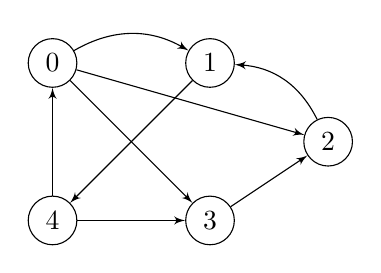
\begin{tikzpicture}
		
		% vertices
		\node[vertex] (a) at  (0,2) {0};
		\node[vertex] (b) at  (2,2) {1};
		\node[vertex] (c) at  (3.5,1) {2};
		\node[vertex] (d) at  (2,0) {3};
		\node[vertex] (e) at (0,0) {4};
		
		%edges
		\draw[edge] (a) to[bend left] (b);
		\draw[edge] (a) to (c);
		\draw[edge] (a) to (d);
		\draw[edge] (b) to (e);
		\draw[edge] (c) to[bend right] (b);
		\draw[edge] (d) to (c);		
		\draw[edge] (e) to (a);
		\draw[edge] (e) to (d);
	\end{tikzpicture}
\end{document}

